\section{Mise en œuvre de la méthode de résolution par intervalles}



\subsection{Algorithmes}
La méthode de résolution par intervalles  met en oeuvre deux opérations détaillées dans \cite{Neumaier}: \\
%\begin{itemize}
%\item{Branch}
\paragraph{Branch :}
\begin{quote}Diviser pour mieux régner\end{quote} Cette méthode consiste à diviser récursivement un problème en deux sous problèmes. Appliquée à la méthode de résolution par intervalles, on découpe en deux l'intervalle concerné (en son milieu ou non). On obtient alors deux problèmes plus «petits» à étudier.\clearpage
%\item{Prune}\\

\paragraph{Prune :}
La découpe d'un problème en sous problèmes peut amener à une situation ou un des sous problèmes créés ne contient aucune solution. On peut alors étudier et trier ces sous problèmes pour en supprimer un espaces de recherche superflu. Cette étape est appelée \textbf{pruning}.
%\end{itemize}
Au bout d'un certain nombre d'itération, l'algorithmes de Branch and Prune propose un ensemble de solutions sous la forme d'intervalles. On visualise sur la figure ci-dessous un tel ensemble dans le cas d'une intersection entre un cercle et d'un disque.

\begin{figure}[h] %on ouvre l'environnement figure
  \center
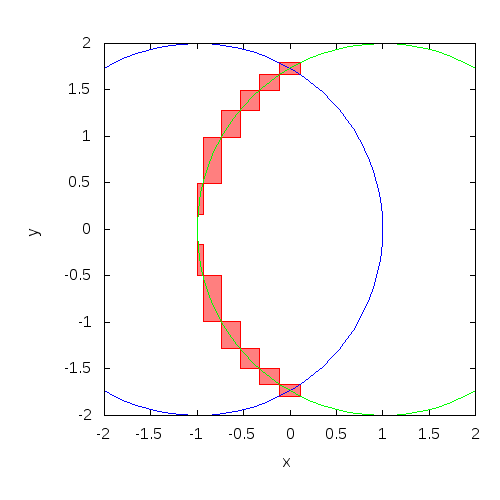
\includegraphics[scale=0.50]{img/circle-disk}
  \caption{Intersection d'un cercle et d'un disque} %la légende
 \label{fig:CercleDisque} %la légende
\end{figure} %on ferme l'environnement figure

\clearpage

\subsection{Données en sortie}
En sortie l'algorithme va nous retourner un ensemble de boîtes. Cet ensemble garantissant, à contrario des méthodes numériques classiques, que toutes les solutions y sont incluses. En voici une illustration dans le cas d'une d'intersections entre deux disques : 
\begin{figure}[h] %on ouvre l'environnement figure
  \center
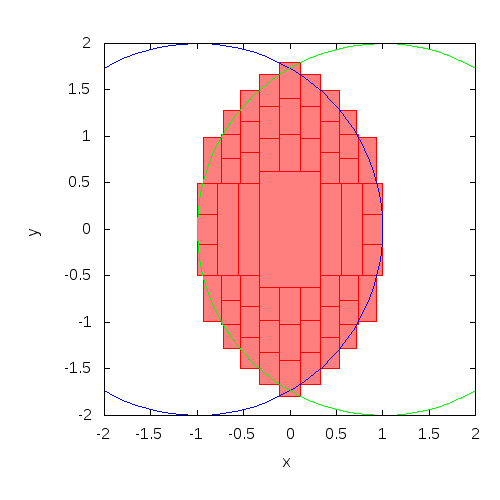
\includegraphics[scale=0.50]{img/disk-disk}
  \caption{Intersection de deux disques} %la légende
 \label{fig:DisqueDisque} %la légende
\end{figure} %on ferme l'environnement figure

 Il est d'ailleurs possible de savoir si tout l'espace d'une boîte est solution du problème. En contrepartie on ne peut toujours garantir l'existence d'une solution dans une enveloppe, il peut donc exister une approximation autour des résultats de l'algorithme.
 \subsection{Outils existant}
\begin{description}
 \item [RealPaver]
\end{description}
